%%%%%%%%%%%%%%%%%%%%%%%%%%%%%%%
%                             %
% Luther Michaels             % 
% ECE 351-52                  %
% Lab 11                      %
% November 18, 2021           %
% Z - Transform Operations    %
%               Lab Report    %
%                             %
%%%%%%%%%%%%%%%%%%%%%%%%%%%%%%%

%%%%%%%%%%%%%%%%%%%%%%%%%%%%%%%%%%%%%%%%%%%
%%% DOCUMENT PREAMBLE %%%
\documentclass[12pt]{report}
\usepackage[english]{babel}
\usepackage{url}
\usepackage[utf8x]{inputenc}
\usepackage{amsmath}
\usepackage{graphicx}
\graphicspath{{images/}}
\usepackage{parskip}
\usepackage{fancyhdr}
\usepackage{vmargin}
\usepackage{listings}
\usepackage{hyperref}
\usepackage{xcolor}
\usepackage{chngcntr}
\usepackage{caption}

\counterwithin*{equation}{section}
\newcommand{\adjust}{\hspace{0.5em}}

\definecolor{codegreen}{rgb}{0,0.6,0}
\definecolor{codegray}{rgb}{0.5,0.5,0.5}
\definecolor{codeblue}{rgb}{0,0,0.95}
\definecolor{backcolour}{rgb}{0.95,0.95,0.92}

\lstdefinestyle{mystyle}{
	backgroundcolor=\color{backcolour},   
	commentstyle=\color{codegreen},
	keywordstyle=\color{codeblue},
	numberstyle=\tiny\color{codegray},
	stringstyle=\color{codegreen},
	basicstyle=\ttfamily\footnotesize,
	breakatwhitespace=false,         
	breaklines=true,                 
	captionpos=b,                    
	keepspaces=true,                 
	numbers=left,                    
	numbersep=5pt,                  
	showspaces=false,                
	showstringspaces=false,
	showtabs=false,                  
	tabsize=2
}

\lstset{style=mystyle}

\setmarginsrb{3 cm}{2.5 cm}{3 cm}{2.5 cm}{1 cm}{1.5 cm}{1 cm}{1.5 cm}

\title{11}	% Title						
\author{Luther Michaels}	% Author		
\date{November 18, 2021}   % Date

\makeatletter
\let\thetitle\@title
\let\theauthor\@author
\let\thedate\@date
\makeatother

\pagestyle{fancy}
\fancyhf{}
\rhead{\theauthor}
\lhead{\thetitle}
\cfoot{\thepage}
%%%%%%%%%%%%%%%%%%%%%%%%%%%%%%%%%%%%%%%%%%%%

\begin{document}
	
%%%%%%%%%%%%%%%%%%%%%%%%%%%%%%%%%%%%%%%%%%%%%%%%%%%%%%%%%%%%%%%%%%%%%%%%%%%%%%%%%%
%%% TITLE PAGE %%%
\begin{titlepage}
	\centering
	\vspace*{0.5 cm}
		
	\begin{center}    
		\textsc{\Large   ECE 351 - Section \#52}\\[2.0 cm]	
	\end{center}  
	\textsc{\Large Z - Transform Operations  }\\[0.5 cm]
	\rule{\linewidth}{0.2 mm} \\[0.4 cm]
	{ \huge \bfseries \thetitle}\\
	\rule{\linewidth}{0.2 mm} \\[1.5 cm]
	\begin{minipage}{0.4\textwidth}
		\begin{flushleft} \large
		\end{flushleft}
	\end{minipage}~
	\begin{minipage}{0.4\textwidth}
		\begin{flushright} \large
			\emph{Submitted By:} \\
			Luther Michaels \break
			
			\emph{Submission Date:} \\
			November 18, 2021
		\end{flushright}
	\end{minipage}\\[2 cm]
\end{titlepage}
	
%%%%%%%%%%%%%%%%%%%%%%%%%%%%%%%%%%%%%%%%%%%%%%%%%%%%%%%%%%%%%%%%%%%%%%%%%%%%%%%%%%
%%% TABLE OF CONTENTS %%%

\tableofcontents
\pagebreak

%%%%%%%%%%%%%%%%%%%%%%%%%%%%%%%%%%%%%%%%%%%%%%%%%%%%%%%%%%%%%%%%%%%%%%%%%%%%%%%%%%
%%% LAB REPORT %%%
\renewcommand{\thesection}{\arabic{section}}
\section{Introduction}
		  
The main concepts in this lab are discrete systems and Z-transforms. The goal is derive the transfer function of a discrete equation and analyze its components and behavior using Python. The various characteristics can be represented visually in a pole-zero plot and a graph of the magnitude and phase frequency response. \\

This procedure relies on the utilization of two Python functions --  scipy.signal.residuez() and scipy.signal.freqz() -- as well as the function zplane() which is provided in the lab manual. The residue function returns the residues, poles, and coefficients for a Z-domain transfer function input. Likewise, the function scipy.signal.freqz() outputs the magnitude and phase response of its Z-domain input as a single variable. The zplane() function developed by Christopher Felton takes a transfer function in the Z-domain, identifies its poles and zeros, and creates a labeled plot of the information. All outcomes and plots can be produced through proper hand-derivation and Python implementation written within the Spyder software. \\

\section{Equations}

\begin{equation}
	y[k] = 2x[k] - 40x[k - 1] + 10y[k - 1] - 16y[k - 2]
\end{equation}
\begin{equation}
	H(z) = \frac{2z^2 - 40z}{z^2 - 10z + 16}
\end{equation}
\begin{equation}
	H(z) = \frac{6z}{z - 2} - \frac{4z}{z - 8}
\end{equation}
\begin{equation}
	h[k] = (6(2)^k - 4(8)^k)u[k]
\end{equation}
\begin{equation}
	|H(z)|\adjust [dB] = 20\cdot log_{10}(|H(z)|)
\end{equation}

\section{Methodology}

The first task in the lab manual requested that the Z-domain transfer function H(z) be found by hand. Beginning with Equation 1, this derivation is shown below.

\begin{equation}
	y[k] = 2x[k] - 40x[k - 1] + 10y[k - 1] - 16y[k - 2]
\end{equation}
\begin{equation*}
	y[k] - 10y[k - 1] + 16y[k - 2] = 2x[k] - 40x[k - 1]
\end{equation*}
\begin{equation*}
	Y(z) - 10z^{-1}Y(z) + 16z^{-2}Y(z) = 2X(z) - 40z^{-1}X(z)
\end{equation*}
\begin{equation*}
	Y(z)[1 - 10z^{-1} + 16z^{-2}] = X(z)[2 - 40z^{-1}]
\end{equation*}
\begin{align}
	H(z) = \frac{Y(z)}{X(z)} &= \frac{2 - 40z^{-1}}{1 - 10z^{-1} + 16z^{-2}} \nonumber \\
	&= \frac{2z^2 - 40z}{z^2 - 10z + 16}
\end{align}

Building from the prior derivation, Task 2 required that the discrete transfer function h[k] be found through partial fraction expansion. The following derivation shows this process, continuing from where the prior task left off.

\begin{equation*}
	\frac{H(z)}{z} = \frac{2z - 40}{z^2 - 10z + 16} \\
\end{equation*}
\begin{equation*}
	\frac{2z - 40}{(z - 2)(z - 8)} = \frac{A}{z - 2} + \frac{B}{z - 8} \\
\end{equation*}
\begin{equation*}
	A = \frac{2z - 40}{z - 8}|_{z = 2} = 6
\end{equation*}
\begin{equation*}
	B = \frac{2z - 40}{z - 2}|_{z = 8} = -4
\end{equation*}
\begin{equation}
	H(z) = \frac{6z}{z - 2} - \frac{4z}{z - 8}
\end{equation}
\begin{equation}
	h[k] = (6(2)^k - 4(8)^k)u[k]
\end{equation}

The third task asked that the function scipy.signal.residuez() be used to verify the results of the partial fraction expansion shown in Equation 3. The numerator and denominator of Equation 2 were implemented as matrices in Python. These two matrices were then used as the input to the Z-transform residue function. The residues, poles, and coefficients returned from this function were then printed to the console and compared with the results of the hand-derivation. \\ 

The fourth task was to use the zplane() function provided in the lab procedure to plot the poles and zeros of the transfer function H(z). The function was copied directly into the lab Python environment, correcting improper alignment and replacing any invalid symbols. The numerator matrix created in the prior task was then reassigned in accordance with $ \frac{H(z)}{z} $, removing the zero term. Given that dividing Equation 2 by $ z $ only affects the numerator, the denominator matrix remained unchanged. These two matrices were then input to zplane() which plotted the pole-zero graph of H(z). \\

Task 5 required the function scipy.signal.freqz() be used to obtain a Bode plot of H(z). The updated numerator and denominator utilized in the prior task were input to this function. The optional condition \textit{whole} was provided a \textit{True} value in order to plot the magnitude and phase across a frequency ranged bounded by zero and the sampling frequency. The default sampling frequency of $ 2\pi\adjust\frac{radians}{sample} $ was used. \\

The Python function returned the frequency range and a complex variable containing the magnitude and phase components. The magnitude was converted to decibels using Equation 5 and numpy.abs() to isolate the magnitude from the complex variable. The phase was likewise assigned to a variable with numpy.angle(). The magnitude and phase response for H(z) was then plotted using commands in the matplotlib.pyplot package to define and arrange the graph as well as provide a title and labels. As the frequency was returned by the function, a step size did not need to be defined for good plot resolution. \\

Github Link: \url{https://github.com/Luther-Michaels} \\

\section{Results}

The Z-domain transfer function H(z) was determined to be given by the equation shown below. The system was assumed to initially be at rest. The Z-transforms of each individual term of Equation 1 were properly transferred from the table of transforms in the textbook. The manipulation of the equation to find the ratio of Y(z) and X(z) preserved the powers of $ z $ and term coefficients. As the accuracy of remaining steps is dependent on H(z), any verification of their results will necessarily support the accuracy of this derivation. 
\begin{equation*}
H(z) = \frac{2z^2 - 40z}{z^2 - 10z + 16}
\end{equation*}

The discrete form of the transfer function was derived to be the following equation. This result is the direct Z-transform of Equation 3, and each term has been properly transferred from the table. The fact that a $ z $ factor is present in the numerator of Equation 2 supports the lack of any shift. The Z-domain step reveals the function's residues to be $ 6 $ and $ -4 $ and its poles to be $ 2 $ and $ 8 $. These results will be verified through a comparison with those printed using a Python package residue function. The residues and poles are also present in the final discrete equation as coefficients and bases as we expect.
\begin{equation*}
	h[k] = (6(2)^k - 4(8)^k)u[k]
\end{equation*}

The printed output from the function scipy.signal.residuez() is provided in the Appendix. The important returned values were the residues of $ 6 $ and $ -4 $ and the poles of $ 2 $ and $ 8 $. These results perfectly match those found from Equations 3 and 4 discussed above. This serves to verify the hand-calculated partial fraction expansion while simultaneously suggesting that the transfer function was properly input in Python as two matrices. The poles in these results will receive further backing via the pole-zero graph of the transfer function. \\

The pole-zero plot of H(z) produced by the zplane() function is shown below. Based on the chart key, we can identify two poles at what appear to be $ 2 $ and $ 8 $. This corroborates part of the results of the prior two tasks given that the poles are the same. The single zero is shown at $ 20 $. This value can be verified by plugging $ 20 $ into Equation 3 which will reduce to zero as we expect. It is notable that the two poles lie in the left half of the complex plane.

\begin{figure}[h]
	\begin{center}
		\caption*{\small \adjust Task 4: Pole-Zero Plot for H(z)}
		\vspace*{-0.43 cm}
		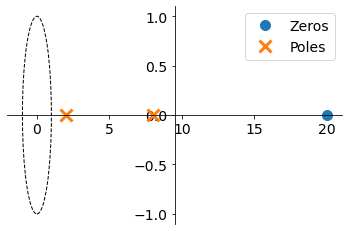
\includegraphics[scale = 0.8]{Lab 11 - Plots/Task4.png}\\[0.5 cm]
	\end{center}
\end{figure}

The following Bode plot of H(z) shows the magnitude and phase over the frequency range provided by scipy.signal.freqz(). This interval runs between $ 0 $ and $ 2\pi $, as we would expect, given that the \textit{whole} option set the upper limit equal to the default sampling frequency of $ 2\pi $. The plots are not shown over a logarithmic scale due to this interval. The magnitude reveals that the transfer function response can be modeled as a band reject filter. At a frequency of $ \pi $, the magnitude takes the value of $ 4 $ while the phase becomes $ 0 $. The phase is given in radians which makes sense as it was plotted directly as the function output. \\

\begin{center}
	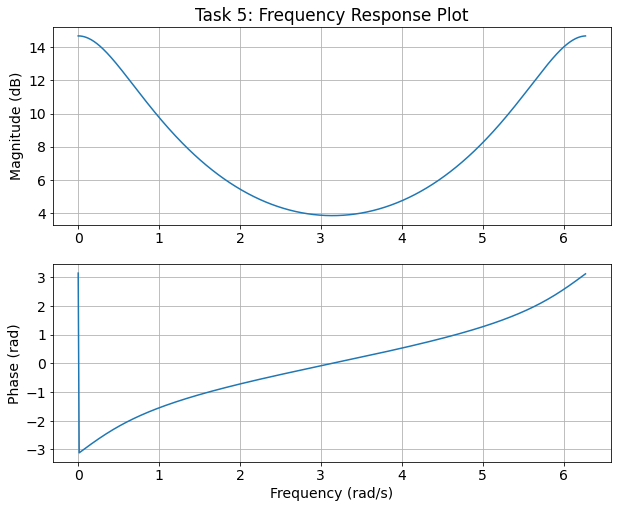
\includegraphics[scale = 0.56]{Lab 11 - Plots/Task5.png}\\[0.5 cm]
\end{center}

\section{Error Analysis}

I initially had difficulty in determining how the numerator input should be arranged between Tasks 3 and 4 to meet the Python functions' requirements. This was particularly an issue given that the provided zplane() function did not seem to document its input form. I solved this problem by observing the pole-zero plot output and comparing the poles and zero with the results of the prior tasks. I discovered that the $ z $ would have to be divided out for the zplane() function input. \\

I also struggled in obtaining a proper phase plot at first. With the help of the TA, I learned that my reassignment of the numerator array in Task 4 could not include an initial zero term. This was due to the fact that I did not create new numerator and denominator matrices. I also did not update the denominator with the numerator. \\

\section{Questions}

1. If we look at the plot generated in Task 4, it is clear that H(z) is stable. As noted in the Results section, all the poles are in the left half of the plane. We learned in a previous lab that this is an indicator of a stable function. This is supported by its discrete form in Equation 4 which contains a negative term of a higher base than the positive. This negative term will keep the function from growing without bound. \\

2. The lab tasks, expectations, and deliverables were all presented clearly. \\

\section{Conclusion}

In this lab we analyzed a discrete system through derivation of its transfer function in the Z-domain and its discrete transfer function. This process taught us the ways in which the partial fraction expansion method differs for Z-domain functions. We used these equations to better understand the relationship between poles and stability as well as to learn about the system's frequency response. \\

If this lab were to be repeated, I would implement a metric to verify the results of the magnitude and phase plot for H(z). As it is now, we can only draw conclusions from the plot. Throughout these labs it has become clear that the best way to understand results is to have some method of adjudicating their validity. This lab allowed us to better our skills in analyzing and understanding the information a graph is presenting through the pole-zero plot. It required us to read function documentation and understand a provided function. This analysis practice will be of great value in improving the rate at which new material may be understood. \\

\newpage
\appendix
\section*{Appendix - Print Output}

Task 3:
\begin{center}
	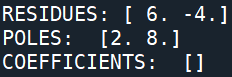
\includegraphics[scale = 1.5]{Lab 11 - Print Output/Task3.png}\\[1.0 cm]
\end{center}

\newpage
\begin{thebibliography}{111}
	
	\bibitem{S}
	Sullivan, Dennis M. (2018) {\it  Signals and Systems for Electrical Engineers I}. Nevada: CreateSpace Independent Publishing Platform.
	
\end{thebibliography}
\end{document}

% Lab Report based on template created by Roza Aceska.